\documentclass[12pt]{article}
%% arXiv paper template by Flip Tanedo
%% last updated: Dec 2016



%%%%%%%%%%%%%%%%%%%%%%%%%%%%%
%%%  THE USUAL PACKAGES  %%%%
%%%%%%%%%%%%%%%%%%%%%%%%%%%%%

\usepackage{amsmath}
\usepackage{amssymb}
\usepackage{amsfonts}
\usepackage{graphicx}
\usepackage{xcolor}
\usepackage{nopageno}
\usepackage{enumerate}
\usepackage{parskip}
\usepackage{framed}
\usepackage{bbm}

\usepackage{sectsty}
\sectionfont{\Large}
% \renewcommand{\thesection}{}
% \renewcommand{\thesubsection}{\arabic{subsection}}

%%%%%%%%%%%%%%%%%%%%%%%%%%%%%%%%%%%%%%%%%%%%%%%
%%%  PAGE FORMATTING and (RE)NEW COMMANDS  %%%%
%%%%%%%%%%%%%%%%%%%%%%%%%%%%%%%%%%%%%%%%%%%%%%%

\usepackage[margin=2cm]{geometry}   % reasonable margins

\graphicspath{{figures/}}	        % set directory for figures

% for capitalized things
\newcommand\acro[1]{{\small {#1}}}

\numberwithin{equation}{section}    % set equation numbering
\renewcommand{\tilde}{\widetilde}   % tilde over characters
\renewcommand{\vec}[1]{\mathbf{#1}} % vectors are boldface

\newcommand{\dbar}{d\mkern-6mu\mathchar'26}    % for d/2pi
\newcommand{\ket}[1]{\left|#1\right\rangle}    % <#1|
\newcommand{\bra}[1]{\left\langle#1\right|}    % |#1>
\newcommand{\Xmark}{\text{\sffamily X}}        % cross out

\let\olditemize\itemize
\renewcommand{\itemize}{
  \olditemize
  \setlength{\itemsep}{1pt}
  \setlength{\parskip}{0pt}
  \setlength{\parsep}{0pt}
}


% Commands for temporary comments
\newcommand{\comment}[2]{\textcolor{red}{[\textbf{#1} #2]}}
\newcommand{\flip}[1]{{\color{red} [\textbf{Flip}: {#1}]}}
\newcommand{\email}[1]{\texttt{\href{mailto:#1}{#1}}}

\newenvironment{institutions}[1][2em]{\begin{list}{}{\setlength\leftmargin{#1}\setlength\rightmargin{#1}}\item[]}{\end{list}}


\usepackage{fancyhdr}		% to put preprint number



% Commands for listings package
%\usepackage{listings}      % \begin{lstlisting}, for code
%
% \lstset{basicstyle=\ttfamily\footnotesize,breaklines=true}
%    sets style to small true-type



%%%%%%%%%%%%%%%%%%%
%%%  HYPERREF  %%%%
%%%%%%%%%%%%%%%%%%%

%% This package has to be at the end; can lead to conflicts
\usepackage{microtype}
\usepackage[
	colorlinks=true,
	citecolor=black,
	linkcolor=black,
	urlcolor=green!50!black,
	hypertexnames=false]{hyperref}





\begin{document}


\begin{center}

    {\Large \textsc{Long HW 4}:
    \textbf{Adventures in Function Space}}
    
\end{center}

\vskip .4cm

\noindent
\begin{tabular*}{\textwidth}{rl}
	\textsc{Course:}& Physics 017, \emph{Linear Algebra for Physics} (S2022)
	\\
	\textsc{Instructor:}& Prof. Flip Tanedo (\email{flip.tanedo@ucr.edu})
	\\
	\textsc{Due by:}& \textbf{Thursday}, May 26
\end{tabular*}

\noindent
This is the `long' assignment assigned every two weeks. You should aim to complete it within two weeks because you'll have new assignments by then, but the formal due date is two weeks + two days. Your explainer video assignment will be to present one of these problems.

If a problem is really thorny, check to make sure the professor did not make a mistake.

% Part of the challenge of the `long' homework may be to figure out exactly what is being asked. Be sure to use the beginning of lecture (or office hours) to ask early when you are confused. Sometimes we are \emph{intentionally} using jargon that you may not be familiar with in order to encourage you to ask and/or look things up.\footnote{Sometimes this is just because the professor is absent minded about what students know and do not yet know.} A good mantra that was once told to the professor when he was a student: \emph{There are no stupid questions. Only stupid students who do not ask questions when they are confused.}

\section*{Reminders about Function Space}

A function space is defined over some interval $a\leq x \leq b$ with sound boundary conditions on the function at $a$ and $b$. The inner product on function space is
\begin{align}
	\langle f, g\rangle = \int_a^b dx\, f(x)^*g(x) \ ,
\end{align}
where $f(x)^*$ is the complex conjugate of $f(x)$. (This is, of course, only relevant for functions that are complex.)


\section{Legendre Polynomials}
% From Griffiths, linear algebra chapter

\begin{figure}[h]
\centering
\includegraphics[width=.3\textwidth]{figures/Legendre_fromWiki.jpg}
\caption{Caricature of Adrien--Marie Legendre by Julien--L\`eopold Boilly (1820); image via Wikipedia (Adrien--Marie Legendre). I think this is the face Legendre makes when someone says, ``your functions aren't normalized.''}
\end{figure}

The first few Legendre polynomials are a polynomial basis for functions defined from $-1\leq x \leq 1$.
\begin{align}
	P_0(x) &= 1 
	& 
	P_1(x) &= x
	&
	P_2(x) &= \frac{1}{2}\left(3x^2-1\right)
	&
	P_3(x) &= \frac{1}{2}\left(5x^3 - 3x\right) \ .
\end{align}
These polynomials are orthogonal, but unfortunately they are not normalized:
\begin{align}
	\int_{-1}^1 P_n(x)^2 \neq 1 \ .
\end{align}
\subsection{Normalized Legendre Polynomials}

A nice basis of functions on $[-1,1]$ should be orthonormal. Define the normalized Legendre polynomials as
\begin{align}
	|0\rangle &= 
	\mathcal N_0
	P_0(x)
	& 
	|1\rangle &= 
	\mathcal N_1
	P_1(x)
	&
	|2\rangle &= 
	\mathcal N_2
	P_2(x)
	&
	|3\rangle &= 
	\mathcal N_3
	P_3(x)
	& \cdots
\end{align}
For the first four Legendre polynomials, explicitly work out what the normalization factors $N_n$ are. \textsc{Answer:} you should find $\mathcal N_n = \sqrt{n+1/2}$.

\subsection{Gram--Schmidt}

The `natural' basis for polynomials are functions $x^n$ for $n=0,1,2,\cdots$. These are neither normalized nor orthogonal on our space. However, they first two such polynomials coincide with the Legendre polynomials. Suppose you started with the first two \emph{normalized} Legendre polynomials, $|0\rangle$ and $|1\rangle$. Perform the Gram--Schmidt procedure to derive the third normalized Legendre polynomial, $|2\rangle$. The steps are:
\begin{enumerate}
\item You know that the next basis element is quadratic, so start with the vector/polynomial $|2'\rangle = x^2$. This vector is not orthonormal with respect $|0\rangle$ and $|1\rangle$. 
\item Find the components of $|2'\rangle$ along $|0\rangle$ and $|1\rangle$. You should find that there is no component of $|2'\rangle$ along $|1\rangle$, but $\langle 2', 0\rangle = (2/3)\mathcal N_0$. 
\item Define a new vector $|2''\rangle$ where you take $|2'\rangle$ and subtract off the component along $|0\rangle$:
\begin{align}
	|2''\rangle = |2'\rangle - \langle 2', 0\rangle |0\rangle \ .
\end{align}
Write out $|2''\rangle$ as a polynomial. This should now be orthogonal to both $|0\rangle$ and $|1\rangle$. (Check that this is true if it is not immediately obvious.)
\item Define  $|2\rangle = C|2''\rangle$, where $C$ is a normalization factor that ensures $\langle 2, 2 \rangle = 1$.
\item Confirm that $|2\rangle = \mathcal N_2 P_2(x)$. 
\end{enumerate}
\textsc{Hint:} be careful to keep track of the normalizations, specifically powers of $\mathcal N_0$.



% You may be curious how to prove the general statement that $N_n=\sqrt{n+1/2}$. There is a recursion relation called the Rodrigues formula that gives a closed form expression for the Legendre polynomials. That gives a shortcut for making general statements the $n^\text{th}$ Legendre polynomial without having to explicitly derive the first $(n-1)$ Legendre polynomials. 

\section{Rodrigues Formula}
% Griffiths QM, sec 4.1
There is a recursion relation called the Rodrigues formula that gives a closed form expression for the Legendre polynomial:
\begin{align}
	P_n(x) = \frac{1}{2^n n!} \left(\frac{d}{dx}\right)^n (x^2 - 1)^n \ .
\end{align}
\subsection{Check it}
Explicitly check that the first four Legendre polynomials match what is predicted by the Rodrigues formula.

\subsection{Orthonormality of Legendre Polynomials, once again}
 
 Use the Rodrigues formula to derive the orthonormality condition for Legendre polynomials:
 \begin{align}
 	\int_{-1}^1 P_n(x)P_m(x) = \frac{2}{2n+1} \delta_{mn} \  .
 \end{align}
 \textsc{Hint:} use integration by parts. 
 

\section{A Laplacian in the wild}

\begin{figure}[h]
\centering
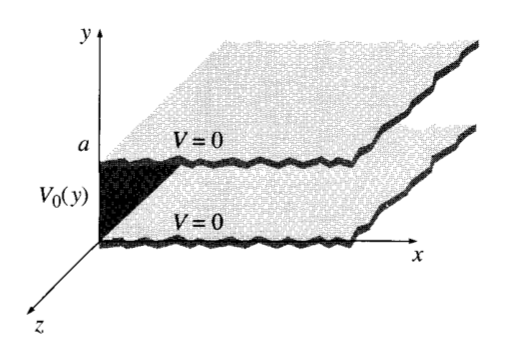
\includegraphics[width=.3\textwidth]{figures/GriffithsEM3-17.png}
\caption{From Griffiths, \emph{Introduction to Electrodynamics}, Example 3.3. }
\label{fig:grif}
\end{figure}

Here's an example from electrodynamics, courtesy of Griffiths' textbook. Two infinite grounded metal plates are parallel to the $xz$ plane: one at $y=0$ and the other at $y=a$; see Fig.~\ref{fig:grif}. The left end, at $x=0$, is closed off with an infinite strip insulated from the two plates and maintained at a specific potential, $V_0(y)$. Find the potential inside the slot.

We will work through this problem systematically from the perspective of Fourier transforms.  Because the system is independent of $z$, the problem boils down to a two-dimensional Laplace equation:
\begin{align}
	\frac{\partial^2V}{\partial^2x}+
	\frac{\partial^2V}{\partial^2y}
	= 0 \ .
\end{align}
\textsc{Comment:} the fact that there is no $\partial^2 V/\partial z^2$ term should be \emph{obvious}, make sure you stop to have an intuition for this. The system is completely symmetric with respect to shifts in the $z$-direction. It looks identical if you pick $z=0$ or $z=23$. That means that the potential $V(x,y,z)$ \emph{cannot} change if you only change $z$.

\subsection{Boundary Conditions, 1}

Explicitly write out the boundary conditions on $V(x,y)$. \textsc{Partial answer:} The tricky one is the boundary at $x\to \infty$. For this one we expect the potential to go to zero, $V(x\to \infty) = 0$. 


\subsection{Boundary Conditions, 2: Separation of Variables}

Make the following ansatz for the solution:
\begin{align}
	V(x,y) = X(x) Y(y) \ .
\end{align}
Rewrite the boundary conditions as conditions on the functions $X$ and $Y$.

\subsection{Separation of Variables}
Given the separation of variables ansatz, $V(x,y)=X(x)Y(y)$, show that the Laplace equation separates; that is, it can be written as:
\begin{align}
	\frac{1}{X}\frac{d^2X}{dx^2}
	= -
	\frac{1}{Y}\frac{d^2Y}{dy^2} \ .
	\label{eq:separation:laplace:result}
\end{align}


\subsection*{Discussion: Reduction to two separate equations}

This is the actual cleverness of the separation of variables method. The two sides of \eqref{eq:separation:laplace:result} are equal to each other. However, they are functions of completely different variables. The left-hand side depends on $x$, whereas the right-hand side depends on $y$. 

If we change $y$, then we expect the right-hand side to change, but not the left-hand side. That would break the equality. This means that the only way for the equality to hold is if both sides are constant and equal to one another. In other words:
\begin{align}
	\frac{1}{X}\frac{d^2X}{dx^2}
	&=
	k^2
	&
	\frac{1}{Y}\frac{d^2Y}{dy^2} 
	&= - k^2 \ .
	\label{eq:laplace:k2}
\end{align}
Here we \emph{chose} to call the constant $k^2$ and we \emph{chose} to put the minus sign on the $Y$ equation. In fact, this came with a bit of foresight. The solutions to the $X$ equation are exponentials, $X(x)\sim e^{\pm k x}$. Since we want $V(x\to \infty,y)=X(x\to\infty)Y(y) \to 0$, it makes sense that the decaying exponential is the `correct' answer for $X(x)$:
\begin{align}
	X(x) \sim e^{-kx} \ .
\end{align}
We do not yet know what the $k$ should be.


\subsection{Fourier Series}
The $Y$ equation is
\begin{align}
	\frac{d^2Y}{dy^2} = -k^2 Y \ .
\end{align}
This is precisely an eigenvalue equation for the second derivative (one dimensional Laplacian). Based on the boundary conditions of this problem, what is the appropriate set of basis functions $|n\rangle = Y_n(y)$ for this equation? Define what the index $n>1$ is indexing.\footnote{You may want to argue why the integers $n>1$ are sufficient to index these basis functions. Why not any negative integers?}

\textsc{Hint}: it is a Fourier series. Are they sines? Cosines? Both? Explain why. The argument of the trigonometric function is $ky$. What condition does the boundary condition place on the allowed values of $k$? You should end up with an infinite number of possible values of $k$. Label these as $k_n$, and give an explicit formula for $k_n$.

% For simplicity, let us call these functions $|n\rangle = Y_n(y)$ for $n>1$. Argue why we only need integers $n>1$, and not negative.

\subsection*{Discussion: the last boundary condition}

You have now found that there are an infinite number of possible $Y(y)$ functions, each characterized by a different wave number $k_n$. However, we know that this wave number also shows up in the $X(x)$ equation. So for each wave number, a valid solution to \eqref{eq:separation:laplace:result}
\begin{align}
	C_n e^{-k_n x} |n\rangle \ .
\end{align}
% (I have spoiled an earlier part of this problem and told you that the answer is $Y\sim \sin$.) 
Here we recall that $|n\rangle = Y_n(y)$ and depends on $k_n$.
So far, $V$ is a sum of these solutions: 
\begin{align}
	V(x,y) = \sum_n C_n e^{-k_n x} |n\rangle
\end{align}
But what are the coefficients, $C_n$? Let's solve for them.

We have one more boundary condition to impose: the $V(x=0,y) = V_0(y)$. For simplicity, let us call this function $|V_0\rangle$ since it is a vector in the space of functions of $y$ from $0\leq y \leq a$. Fortunately, we just derived a nice basis for this function space. To impose the boundary condition, use the orthonormality of the basis $|n\rangle$. Multiply both sides of the boundary condition by one:
\begin{align}
	\mathbbm{1} = \sum_m |m\rangle \langle m| \ .
\end{align}
This gives:
\begin{align}
	\sum_m |m\rangle \langle m|
	\sum_n \left.C_n e^{-k_n x} |n\rangle\right|_{x=0}
	= 
	\sum_m |m\rangle \langle m| V_0\rangle
	\label{eq:fourier}
\end{align}
Since the basis elements are orthonormal, we have
\begin{align}
	C_n |m\rangle = \langle m| V_0\rangle \ .
\end{align}
Make sure it is obvious how we `got rid' of the sum over $m$ in this step! If it helps, you can imagine projecting onto a particular value of $m$ by hitting both sides of \eqref{eq:fourier} by $\langle m'|$.

\subsection{Solving the problem}

Consider the case where $V_0(y) = V_0$, a constant. Explicitly solve for the coefficients $C_n$. \textsc{Answer:}
\begin{align}
	C_n = 
	\begin{cases}
	0 & \quad\text{if $n$ is even} \\
	\frac{4V_0}{n\pi} &\quad\text{if $n$ is odd} 
	\end{cases} \ .
\end{align}










\section{Angular Momentum}

In quantum mechanics, the wavefunction of a particle encodes everything there is to know about it. Observable (measurable) properties of the particle are the eigenvalues of Hermitian operators. For example, momentum is identified with the gradient, $\vec{p} = -i\hbar \nabla$. In other words, $p_x = -i\hbar \partial_x$. 

\subsection{Momentum of a plane wave}

A plane wave has a wavefunction
\begin{align}
	\psi(x,t) \sim e^{i(kx - \omega t)} \ .
\end{align}
What is the momentum of this plane wave? \textsc{Discussion}: yes, it is obvious from the way we wrote the right-hand side. Please argue based on the statement that the observed momentum is the eigenvalue of the momentum operator.

\subsection{Hermiticity of the momentum}

An operator $\mathcal O$ is Hermitian if $\mathcal O^\dag = \mathcal O$. That means:\footnote{This comes from the definition of $\mathcal O^\dag$ as $\langle \psi, \mathcal O^\dag \chi \rangle = 
	\langle \mathcal O \psi,\chi \rangle$.}
\begin{align}
	\langle \psi, \mathcal O \chi \rangle = 
	\langle \mathcal O \psi,\chi \rangle
\end{align}
Given the form of the inner product on function space, is the momentum operator Hermitian? Is $\partial_x$ Hermitian? Explain the significance of the factor of $i$ in the definition of the momentum operator. 

\subsection{Momentum and Angular Momentum in Quantum Mechanics}

In classical mechanics, angular momentum is $\vec L = \vec{r} \times \vec{p}$. This has components:
\begin{align}
	L_x &= yp_z -zp_y 
	&
	L_y &= zp_x - xp_z
	&
	L_z &= xp_y - yp_x \ .
\end{align}
In quantum mechanics, the components of the angular momentum operator are the same, but with $p_i \to -i\hbar \partial_i$. 

The angular momentum operator is the \emph{generator of rotations}. Recall from earlier long homework that the generator of a transformation is the infinitesimal realization of that transformation. You have already worked out the commutation relations for the generators of rotations on these past homework. Now you can do it one more time.

Show that the commutation relations of the components of the angular momentum operator satisfy
\begin{align}
	[L_x, L_y] = i\hbar L_z \ .
	\label{eq:LxLy}
\end{align}
That should look \emph{really} familiar from your past homework.

\textsc{Hint}: working out the commutation relations of a differential operator can be tricky. To do it properly, you need to provide a test function, $f(x,y,z)$. To prove \eqref{eq:LxLy}, you should act on this test function 
\begin{align}
	[L_x, L_y]f = (-i\hbar)^2
	\left[\left(y\partial_z - z\partial_y\right)
	\left(z\partial_x - x\partial_z\right)f
	-
	\left(z\partial_x - x\partial_z\right)
	\left(y\partial_z - z\partial_y\right)
	f
	\right] \ .
\end{align}
Be careful with the chain rule. For example: the first term on the right-hand side is
\begin{align}
	(-i\hbar)^2 y\partial_z\left(z\partial_x f\right)
	= 
	y\partial_xf + yz\partial_z\partial_xf\ .
\end{align}
You can use the fact that mixed partial derivatives commute so that $\partial_x\partial_yf = \partial_y\partial_xf$.

\section{Some commutation relations}

The results of this problem are useful for subsequent problems. Do not use the differential operator or matrix formulation of the angular momentum operator to do these problems (although the results will still be true). Instead, just use the commutation relations of the $L_i$. 

\subsection{Commutator identity}

Prove the following identity for commutators:
\begin{align}
	\left[AB,C\right] = A[B,C] + [A,C]B \ .
\end{align}

\subsection{Commuting observables}

The total angular momentum (squared) is $L^2 = L_x^2 + L_y^2 + L_z^2$. You have shown that components of angular momentum do not commute with each other. Show that the total angular momentum commutes with each component:
\begin{align}
	\left[L^2,L_z\right] = 0  .
\end{align}
You can replace $L_z$ by $L_x$ or $L_y$ and the equation is still true.

\textsc{Discussion}: \emph{This is really important:} $[L^2, L_z]=0$ means that $L^2$ and $L_z$ may be simultaneously diagonalized. There is some basis of simultaneous eigenstates of $L^2$ and $L_z$. You can thus use the eigenvalues of $L^2$ and $L_z$ to index the basis functions.

Suppose you have an eigenfunction of both $L^2$ and $L_z$. Because $[L_z,L_x]\neq 0$, the state will \emph{not} be an eigenfunction of $L_x$. This is the mathematical manifestation of the \emph{uncertainty principle}. If you \emph{know} what the $z$-component of angular momentum is\footnote{Here we mean: ``if you are in an eigenstate of $L_z$...''}, then you are uncertain about what the $x$-component will be when you measure the state.\footnote{The usual position--momentum uncertainty relation is $[x,p]\sim \hbar$, where $x$ and $p$ are the operators whose eigenvalues are the position and the momentum of the state.}


\subsection{Ladder operators}

Define the raising and lowering operators:
\begin{align}
	L_\pm \equiv L_x \pm i L_y \ .
\end{align}
Show that these satisfy
\begin{align}
	[L_z, L_\pm] &= \pm \hbar L_\pm
	&
	[L^2, L_\pm] &= 0 \ .
\end{align}
This is easy to check using the commutation relations of the angular momentum operator. You do \emph{not} have to invoke the explicit form of differential operators, just the commutation relations.

\subsection{Raising and Lowering Operators}

% Define the raising and lowering operators
% \begin{align}
% 	L_\pm \equiv L_x \pm i L_y \ .
% \end{align}
Show that
\begin{align}
	L^2 = L_\pm L_\mp + L_z^2 \mp \hbar L_z \ .
	\label{eq:L2:pm}
\end{align}
\textsc{Hint:} Calculate $L_\pm L_\mp$ and then remember the commutation relation for $[L_x, L_y]$.



\section{Quantum Mechanics with Spherical Symmetry}

In systems with spherical symmetry, it is natural to use spherical coordinates. In this case, the Laplacian is a horrible mess. Here it is:
\begin{align}
	\nabla^2
	=
	\frac{1}{r^2}
	\partial_r \left(r^2\partial_r\right)
	+\frac{1}{r^2\sin\theta}\partial_\theta \left(\sin\theta\partial_\theta\right)
	+\frac{1}{r^2\sin^2\theta} \partial_\phi^2 \ .
\end{align}
Look upon this operator and despair!\footnote{``Ozymandias,'' Percy Bysshe Shelley.} Don't worry The material here is standard in most introductory quantum mechanics textbooks. Feel free to take a look at your favorite one if you need some guidance.

\subsection{Separation of Variables}

To solve $\nabla^2 \psi(r,\theta,\phi)=0$, one can again make the separation of variables ansatz: $\psi= R(r), Y(\theta, \phi)$. Show that you end up with:
\begin{align}
	\frac{1}{R}\frac{d}{dr}\left(r^2\frac{dR}{dr}\right)
	= 
	-\frac{1}{Y}
	\left[
	\frac{1}{\sin\theta}\frac{\partial}{\partial \theta}
	\left(\sin\theta \frac{\partial Y}{\partial \theta}\right)
	+ \frac{1}{\sin^2\theta}\frac{\partial^2Y}{\partial\phi^2} 
	\right] \ .
\end{align}
Because each side depends on different variables, they must both be equal to one another. With some foresight, we will call this constant $\ell(\ell+1)$. We will figure out why we did this and what $\ell$ actually is shortly. Note that the angular equation is an eigenvalue equation:
\begin{align}
	\sin\theta \frac{\partial}{\partial_\theta}\left(\sin\theta \frac{\partial Y}{\partial\theta}\right) + \frac{\partial^2 Y}{\partial\phi^2}
	= -\ell(\ell+1)\sin^2\theta \, Y \ .
	\label{eq:Y:l}
\end{align}


\subsection{Separation of variables for the angular function}

We can separate variables again! Write
\begin{align}
	Y(\theta,\phi)=\Theta(\theta)\Phi(\phi) \ .
\end{align}
Show that we end up with
\begin{align}
	\frac{1}{\Theta}
	\left[
	\sin\theta \frac{d}{d\theta}
	\left(\sin\theta \frac{d\Theta}{d\theta}\right)
	\right]
	+ \ell(\ell+1)\sin^2\theta
	= - \frac{1}{\Phi}\frac{d^2\Phi}{d\phi^2} \ .
	\label{eq:sep:Y:phi}
\end{align}
Again, both sides depend on different variables. Therefore both sides must be constant. Let us call this constant $m^2$. 

\subsection{Quantization}

The right-hand side of \eqref{eq:sep:Y:phi} must thus satisfy
\begin{align}
	\frac{1}{\Phi}\frac{d^2\Phi}{d\phi^2} = -m^2 \ .
\end{align}
This looks familiar, right? What are the solutions? You can use trigonometric functions, or a more convenient option is $e^{im\phi}$. Now think about the boundary conditions of the function space that $\Phi(\phi)$ lives in. What is the boundary condition for $\phi=0$ and $\phi=2\pi$? 

Argue that the boundary condition restricts $m$ to be an integer. Congratulations, your system is now manifestly quantized. We call $m$ a quantum number because it takes discrete values.


\subsection*{Discussion: Spherical Harmonics}

The normalized eigenfunctions for the angular part of the Laplacian \eqref{eq:Y:l} are called \textbf{spherical harmonics}. Here's what these bastards look like:
\begin{align}
	Y_\ell^m(\theta,\phi)=
	\epsilon
	\sqrt{\frac{2\ell+1}{4\pi} \frac{(\ell-|m|)^2}{(\ell+|m|)^2}}
	e^{im\phi}
	P_\ell^m(\cos\theta) \ .
\end{align}
The weird objects are:
\begin{align}
	\epsilon &\equiv 
	\begin{cases}
	(-1)^m &\quad\text{for }m> 0\\
	+1&\quad\text{for }m \leq 0  \ .
	\end{cases}
	&
	P_\ell^m(x) 
	&\equiv(1-x^2)^{|m|/2}
	\left(\frac{d}{dx}\right)^{|m|}P_\ell(x) \ ,
\end{align}
the latter functions are called associated Legendre polynomials. 

We note that the $Y_\ell^m$ spherical harmonics have two indices: $\ell$ coming from the separation of variables $\psi = RY$ and $m$ coming from the separation of variables $Y=\Theta\Phi$. We already showed that $m$ is quantized. When you turn the crank (see, e.g. Griffiths \emph{Introduction to Quantum Mechanics}), you end up with the following restrictions:
\begin{align}
	\ell &= 0, 1, 2, \cdots
	&
	m = -\ell, -\ell+1, \cdots, -1, 0, 1, \cdots, \ell-1, \ell \ .
\end{align}

\subsection{Angular momentum of a spherical harmonic}

In spherical coordinates, the angular momentum in the $z$ direction is
\begin{align}
	L_z = -i\hbar \frac{\partial}{\partial\phi} \ .
\end{align}
What is the angular momentum in the $z$ direction of $Y^m_\ell(\theta,\phi)$?




\section{Total angular momentum}

We'd like to figure out what the $\ell$ means in our spherical harmonics.



\subsection{Eigenvalues of raised/lowered functions}

Let $f_{\lambda,\mu}$ be an eigenfunction of $L^2$ with eigenvalue $\lambda$ and simultaneously an eigenfunction of $L_z$ with eigenvalue $\mu$. We are allowed to have such a state because $[L^2, L_z]=0$.

Using the commutation relations above, show that $L_\pm f$ is also an eigenvector of $L^2$ with eigenvalue $\lambda$, and simultaneously an eigenfunction of $L_z$ with eigenvalue $(\mu \pm \hbar)$. 

\textsc{Discussion:} Given a a simultaneous eigenfunction of $L^2$ and $L_z$, we can now generate more eigenfunctions with the same $L^2$ eigenvalue and different $L_z$ values. We say we can construct a \emph{ladder} of states with the same total angular momentum but different angular momentum in the $z$ direction. Given the state $f_{\lambda,\mu}$, we can create states $f_{\lambda,\mu\pm 1} = L_\pm f_{\lambda,\mu}$. Then we can continue upward and downward in values of $m$.

\subsection{Maximum angular momentum in the z direction}

There is a maximum possible rung to this ladder. Physically, the angular momentum in the $z$ direction cannot exceed the total angular momentum. that means there is a `top rung' eigenfunction $f_\text{top}$ such that
\begin{align}
	L_+ f_\text{top} = 0. 
\end{align}
With some foresight, \emph{define} $\ell$ to be the maximum $L_z$ eigenvalue:
\begin{align}
	L_z f_\text{top} &= \hbar \ell f_\text{top}
	&
	&\Rightarrow &
	f_\text{top} =  f_{\lambda,\ell}
	 \ . 
\end{align}
Use \eqref{eq:L2:pm} to show that
\begin{align}
	L^2 f_{\lambda,\ell} = \hbar^2 \ell(\ell+1) f_{\lambda,\ell} \ .
\end{align}
In other words, the eigenvalue of total angular momentum is
\begin{align}
	\lambda = \hbar\ell(\ell+1) \ .
\end{align}

\subsection*{Discussion}
We have now identified $\ell$ as a number that gives the total angular momentum. $m=\ell$ is the maximum angular momentum in the $z$-direction. You can follow the same analysis to determine that there is a minimum $L_z$ eigenvalue, the `bottom rung' of the ladder. What one finds is that the minimum value is $-\hbar \ell$ and that $\ell$ is also quantized to be integer values. The value of $\ell$ is sometimes called the azimuthal quantum number. 

What we have found is that our eigenfunctions of the angular part of the spherical Laplacian, the spherical harmonics, are states with some total angular momentum indexed by $\ell$ and some angular momentum in the $z$ direction indexed by $m$. These functions are orthonormal with respect to integration over the angles of the unit sphere. 

You can solve problems in, say, electrostatics with hemispherical conductors by using a basis of spherical harmonics analogously to the way that we solved the metal conductor problem above using Fourier series. I thought about adding a problem like that to this problem set, but I decided that it would be too cruel.

















\end{document}
